\section{M3 constrained admissible sets}
\label{app:m3-constrained-admissible-sets}

\subsection{The question M3 asks}

M2 showed that two matrix representations can have the same band energies and
retained projector while having very different hopping coefficients. The
difference comes from a momentum-dependent rotation of the retained orbital
frame. A separate rotation at every momentum point recovers the original M2
matrices almost exactly, but one constant rotation over the whole Brillouin zone
generally cannot.

M3 asks a narrower question:
\begin{quote}
Can one reduced Hamiltonian satisfy both the spectral and
represented-operator requirements when the candidate family and allowed
orbital alignments are fixed in advance?
\end{quote}
This is a compatibility question under a declared contract. It is not a claim
that the underlying physical systems are different or that no more general
alignment could reconcile their matrices.

\subsection{A two-knob candidate model}

M3 starts from the transported M2 reference Hamiltonian $H(k)$. Let
$\overline E(k)=\operatorname{tr}H(k)/2$ be its mean band energy. A candidate is
\[
 H_{s,\lambda}(k)
 =\overline E(k)I+sE_GI
 +\lambda\left[H(k)-\overline E(k)I\right],
\]
where $E_G=1$ in the parent energy unit. The two parameters have simple roles:
\begin{itemize}
 \item $s$ shifts both bands together;
 \item $\lambda$ changes their splitting about the mean; and
 \item $(s,\lambda)=(0,1)$ is the original reference model.
\end{itemize}
The frozen search rectangle is
\[
 -0.25\leq s\leq0.25,
 \qquad
 0.4\leq\lambda\leq1.2.
\]
For matrix comparison, M3 allows only nine constant real rotations, with angles
from $-1.2$ to $1.2$ radians. It does not allow the momentum-dependent
pointwise alignment that recovers M2 exactly.

\subsection{Two accepted regions}

Each candidate receives two normalized RMS scores:
\begin{enumerate}
 \item \emph{spectral loss}, measuring disagreement between ordered band
 energies; and
 \item \emph{operator loss}, measuring matrix disagreement after the best
 allowed constant rotation.
\end{enumerate}
A threshold on each score produces a region in the $(s,\lambda)$ plane. The
spectral admissible set contains candidates passing the spectral threshold. The
operator admissible set is the union of the passing regions for the nine
rotation angles.

The decision rule is geometric. A retained point belonging to both regions
proves compatibility. Failure to find such a point proves nothing by itself. A
positive lower bound on the distance between the complete frozen regions
certifies separation.

Only the 64 training points define these regions and their quadratic
boundaries. The 257 staggered evaluation coordinates are disjoint from training
and are used only after the decision objects have been fixed.

\subsection{How the thresholds were chosen}

The thresholds are benchmark-design controls, not physical tolerances. They
were chosen from the known synthetic model and its preparatory analytic
training-loss geometry to produce two deliberately different decision regimes.

\begin{table}[ht]
\centering
\small
\caption{Design roles of the M3 thresholds and resolution.}
\begin{tabular}{@{}p{0.25\linewidth}p{0.67\linewidth}@{}}
\toprule
Control & Design role \\
\midrule
Spectral threshold $0.03$
 & Keeps spectral acceptance near the original splitting and places its
 minimum accepted splitting at approximately $0.9354687052$. \\
Compatible operator threshold $0.33$
 & Lies just above the original model's constrained operator loss
 $0.3286318914$, so $(0,1)$ is a common witness. \\
Separated operator threshold $0.31$
 & Shrinks operator acceptance until its maximum splitting is approximately
 $0.8360013041$. \\
Separation resolution $0.05$
 & Declares the minimum parameter-space gap that this benchmark will call
 resolved. \\
\bottomrule
\end{tabular}
\end{table}

Thus the separated design was required to satisfy
\[
 0.9354687052-0.8360013041
 =0.0994674010>0.05.
\]
The thresholds were frozen before the retained confirmatory execution, but
their selection was not blind. They were not inferred from withheld values,
experimental uncertainty, literature tolerances, or material acceptance
criteria. The calculation therefore demonstrates the decision procedure; it
does not calibrate universal thresholds.

An explicitly post-hoc analytic reanalysis varies only the operator threshold
while holding $\tau_S=0.03$. The operator set first becomes feasible at
approximately $0.307420$. Its distance from the spectral set exceeds the
declared $0.05$ resolution until $\tau_O=0.313791$, remains positive but below
resolution until the exact compatibility transition at $\tau_O=0.319264$, and
is compatible thereafter. The original point $(0,1)$ itself becomes
operator-admissible at $0.328632$. Thus the two designed thresholds lie
transparently on opposite sides of the transition rather than serving as
estimates of a physical tolerance. Its hardened verifier correlates the
consumed M3 result to the exact source-manifest entry and checks the zero-shift,
axis-alignment, symmetry, and positive-curvature premises used by this
reduction.

\begin{figure}[ht]
 \centering
 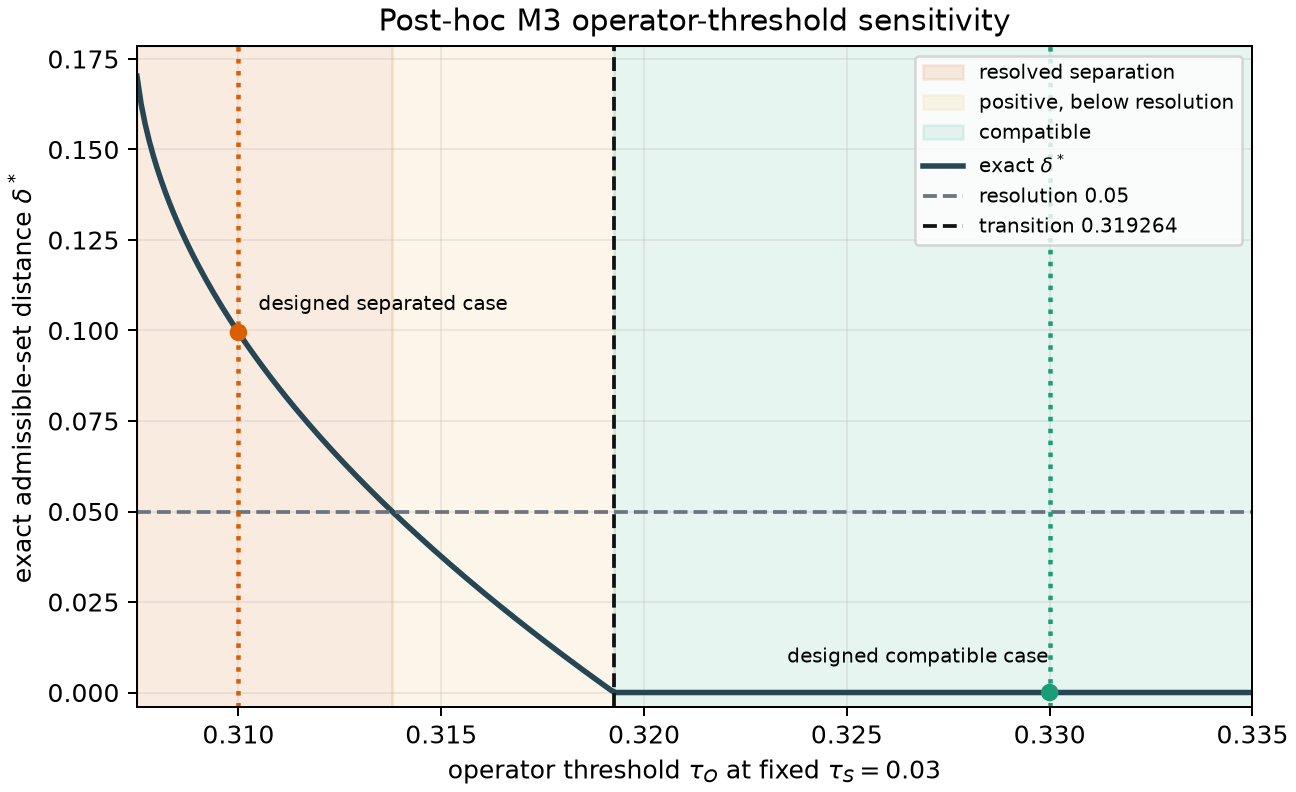
\includegraphics[width=0.96\linewidth]{../../../../../calculations/ICMSEP2026/conference/paper_1/constrained-admissible-sets-threshold-sensitivity/operator-threshold-sensitivity.png}
 \caption{Explicitly post-hoc M3 operator-threshold sensitivity at fixed
 $\tau_S=0.03$. The curve distinguishes resolved separation, positive distance
 below the declared resolution, and compatibility.}
 \label{fig:m3-threshold-sensitivity}
\end{figure}

\subsection{Compatible thresholds}

The first thresholds are
\[
 \tau_S=0.03,
 \qquad
 \tau_O=0.33.
\]
The original model $(0,1)$ passes both tests when the constant rotation angle is
$0.3$:
\begin{itemize}
 \item training spectral loss: $7.59\times10^{-16}$; and
 \item training operator loss: $0.3286318914$.
\end{itemize}
Because M3 retains this explicit common witness, the distance between the two
accepted regions is exactly zero. This is stronger than reporting that a
numerical search happened to find a small loss.

\subsection{Tightened operator threshold}

The second case keeps the spectral threshold at $0.03$ but tightens the operator
threshold to $0.31$. Within the frozen parameter rectangle and nine-angle
alignment family,
\begin{align*}
 \text{spectral acceptance}&:\quad \lambda\gtrsim0.9354687052,\\
 \text{operator acceptance}&:\quad \lambda\lesssim0.8360013041.
\end{align*}
The closest retained boundary points are therefore
\[
 p_S\approx(0,\,0.9354687052),
 \qquad
 p_O=(0,\,0.8360013041).
\]
Their Euclidean distance is
\[
 \lVert p_S-p_O\rVert_2=0.0994674010.
\]
The analytic quadratic certificate gives the same value as both a lower and a
constructive upper bound. Because it exceeds the prospectively frozen
resolution $0.05$, the retained disposition is \emph{certified separated}.

\begin{figure}[ht]
 \centering
 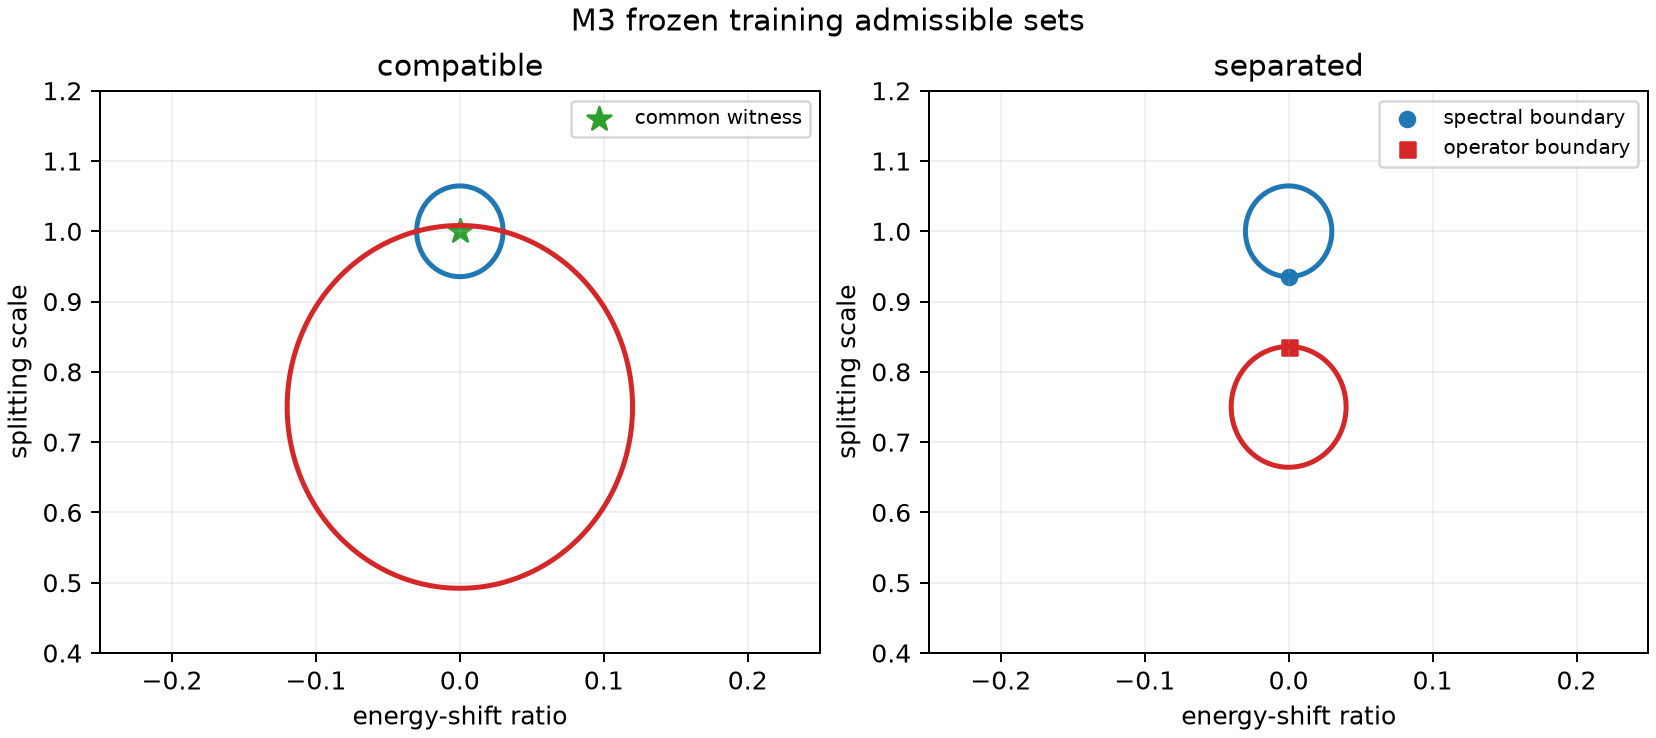
\includegraphics[width=0.96\linewidth]{../../../../../calculations/ICMSEP2026/conference/paper_1/constrained-admissible-sets/constrained-admissible-sets-summary.png}
 \caption{M3 constrained admissible sets. The compatible thresholds admit the
 original model as a common witness. Tightening the operator threshold leaves a
 certified gap between the spectral and operator regions.}
 \label{fig:m3-constrained-admissible-sets}
\end{figure}

\subsection{What the result does and does not mean}

M3 demonstrates that spectral and matrix requirements can select nonoverlapping
parts of the same reduced-model family when the alignment family and tolerances
are fixed. The result depends on the two-parameter model, nine constant
rotations, thresholds, Euclidean metric, finite meshes, and
quadratic-certificate assumptions.

It does not establish material validity, uncertainty quantification, silicon
transferability, or incompatibility under arbitrary momentum-dependent
alignments. In particular, M2 already shows that pointwise alignment can
recover the constructed frame attack almost exactly.

Before confirmatory evaluation, the editable TOML configuration, deterministic
input builder, derived input, M2 input digest, implementation sources, runner,
and standalone verifier were bound by \path{protocol-freeze.json}. Nine
retained amendments record post-freeze corrections and boundary hardening;
amendment 6 retracts an earlier incorrect diagnosis of a shared
training/evaluation coordinate, and amendment 9 records post-result role and
tolerance verification hardening without changing scientific controls or
numerical results.

The library verifier reports maximum dimensionless defect
$1.33\times10^{-15}$. The standalone verifier, which imports no producer
Actions, reports $4.66\times10^{-15}$, below the frozen $10^{-11}$ tolerance.
It nevertheless shares NumPy, SciPy, eigensolvers, floating-point behavior, and
scientific conventions with the producer. SHA-256 binds recorded bytes but does
not independently establish chronology.
